\section{Durchführung}
\label{sec:Durchführung}

Um den Photoeffekt untersuchen zu können, wird eine Photozelle genutzt.
Diese besteht aus einem evakuierten Glaskolben.
Auf diesen ist die sogenannte Photokathode aufgedampft.
Diese wird mit Licht bestrahlt, so dass aufgrund des Photoeffektes Elektronen herausgeschlagen werden.
Diese Elektronen werden von der Anode aufgenommenm welche aus einem dünnen Draht besteht und kreisförmig um die Photokathode konstruiert ist.
Der Aufbau der Photozelle ist in Abbildung \ref{fig:Photozelle} und der der optischen Anordnung in Abbildung \ref{fig:Aufbau} dargestellt.

  \begin{figure}
    \centering
    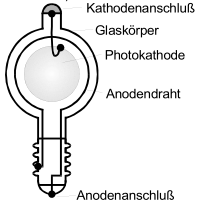
\includegraphics[width=0.5\textwidth]{images/Photozelle.png}
    \caption{Der Aufbau einer Photozelle, entnommen der Veruschsanleitung \cite{sample}.}
    \label{fig:Photozelle}
  \end{figure}
  \begin{figure}
    \centering
    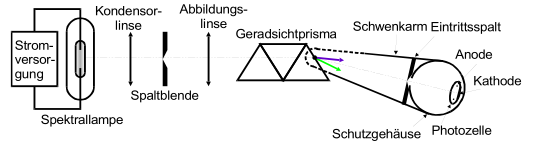
\includegraphics[width=1\linewidth]{images/Aufbau.png}
    \caption{Die optische Anordnung, entnommen der Veruschsanleitung \cite{sample}.}
    \label{fig:Aufbau}
  \end{figure}
  \begin{figure}
    \centering
    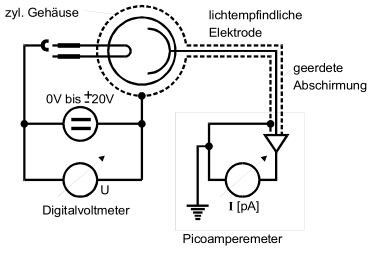
\includegraphics[width=0.7\linewidth]{images/Messung.png}
    \caption{Die Messvorichtung für die Bremsspannung und den Elektronenstrom, entnommen der Veruschsanleitung \cite{sample}.}
    \label{fig:Messung}
  \end{figure}

Die Kondensorlinse bündelt das Licht der Spektrallampe.
Die Abbildungslinse erzeugt ein Bild der Spaltblende auf deb Eintritsspalt der Photozelle.
Das Geradsichtprisma dient der räumlichen Auftrennung des Lichtes, so dass die einzelnen Spektrallinien der Lampe auf die Photozelle gerichtet werden können.
Die Photozelle ist dafür schwenkbar gelagert.
Mithilfe eines Mattschirmes können die Einstellungen der Linsen überprüft werden.
Die Spektrallinien sollten scharf erkennbar sein.

Um die Energie der vom Photoeffekt ausgelösten Elektronen messen zu können wird die Gegenfeldmethode verwendet.
Hierfür wird an die Anode eine variable Spannung angelegt.
Dies erzeugt ein Elektronen abbremsendes Feld.
Es ist nun möglich für verschiedene Spannungen den Elektronenstrom zu messen.
Der Aufbau der Schaltung ist in Abbildung \ref{fig:Messung} dargestellt.

Die einzelnen Spektrallinien werden jeweils auf die Photozelle ausgerichtet.
Es wird ein Bereich von Bremsspannung abgeschätzt, für den sich genügend Messwerte nehmen lassen.
Für jede Bremsspannung wird der Elektronenstrom aufgenommen.
Dies wird für jede Spektrallinie wiederholt.
Besondere Beachtung wird der Wellenlänge $\lambda = \SI{578}{\nano\metre}$ geschenkt.
Für diese werden die Bremsspannungswerte von $ (\SI{-20}{\volt} \leq \text{U} \leq \SI{+20}{\volt})$ aufgenommen.
